\documentclass[11pt,a4paper]{article}

\usepackage[utf8]{inputenc}
\usepackage[T1]{fontenc}
\usepackage{lmodern}
\usepackage[margin=2.5cm]{geometry}
\usepackage{amsmath,amssymb}
\usepackage{graphicx}
\usepackage{xcolor}
\usepackage{booktabs}
\usepackage{tabularx}
\usepackage{array}
\usepackage{caption}
\usepackage[colorlinks=true,linkcolor=blue!45!black,citecolor=blue!45!black,
            urlcolor=blue!45!black,bookmarks=true,bookmarksnumbered=true]{hyperref}

\graphicspath{{../../phase3/ablation/metrics/}{../../phase3/tradeoff/}{../../phase3/l2_llm/}}
\captionsetup{font=small,labelfont=bf}
\setlength{\emergencystretch}{3em}
\renewcommand{\arraystretch}{1.2}

\newcommand{\kp}{\ensuremath{\kappa}}
\newcommand{\code}[1]{\texttt{\small #1}}

\title{}\author{}\date{}

\begin{document}

% ===================== TITLE =====================
\begin{titlepage}
\centering
\vspace*{2.2cm}
{\Large\bfseries Measuring and Mitigating Privacy Leakage\\[4pt]
in Enterprise Retrieval-Augmented Generation\par}
\vspace{1.4cm}
{\large A study of layered defenses, their measured effect,\\ and the residual risk they leave behind\par}
\vspace{2.4cm}
{\rule{0.7\textwidth}{0.4pt}}\\[10pt]
{\large\bfseries TADJ Mohamed Walid}\\[6pt]
{\normalsize Master's in Artificial Intelligence \& Data Science}\\
{\normalsize \'Ecole Sup\'erieure en Informatique (ESI), Sidi Bel Abb\`es}\\
{\normalsize 2025--2026}\\[10pt]
{\rule{0.7\textwidth}{0.4pt}}\\[1.2cm]
{\normalsize Under the supervision of\\[2pt]
Professor Esma A\"imeur \quad and \quad Professor Souleyman Chaib}
\vfill
{\normalsize June 2026}
\end{titlepage}

% ===================== ABSTRACT =====================
\begin{abstract}
\noindent
Enterprise retrieval-augmented generation (RAG) makes an organization's documents conversationally
accessible, and in the same motion exposes the personal information those documents contain. This
report asks how, and how far, that exposure can be reduced. Working against a corpus of 155 synthetic
but realistic records in which every sensitive entity has been annotated in advance, we assemble a
layered privacy defense and then measure it with two independent instruments: a fast rule-based
detector, and a language-model judge whose agreement with human annotators reaches Cohen's
\kp{}~$=0.827$ on undefended text. The two instruments disagree in a way that turns out to be the most
important result of the work. The detector reports that the full defense removes leakage almost entirely; the validated
judge shows that it does not. Read through the judge, the attack-success rate falls from 28.8\% on the
undefended system to 17.3\% with every layer active, a reduction of roughly forty percent rather than
the near-elimination the detector claims, and one carried almost entirely by redaction of personal
data at retrieval time. What survives is re-identification by linkage: an adversary who assembles a
handful of innocuous facts about a person from separate documents is barely impeded by any redaction
layer. One caveat we measure rather than assume: the judge that delivers these figures, though strongly
aligned with human labels on undefended text, agrees far less on defended output (\kp{} falling from
0.827 to 0.306), erring mostly by reading refusals as leaks. It is still the better of the two
instruments --- the detector is worse on the same test --- so the direction and rough size of the
reduction hold even where its exact height is uncertain; and the re-identification leaks it missed were
ones the human caught, which only sharpens the linkage finding. The broader lesson is methodological. Evaluating a RAG privacy defense with a single,
unvalidated detector systematically overstates how well it works. The prototype that accompanies this
study demonstrates the recommended configuration in a live system; it is a demonstration, not a
certified product, and it does not close the linkability gap.
\end{abstract}

\tableofcontents
\newpage

% ===================== 1. INTRODUCTION =====================
\section{Introduction}

A company that has accumulated years of internal records --- personnel files, configuration documents,
internal correspondence, medical reports --- and decides to make them conversationally accessible
faces a problem that is easy to miss. The retriever that fetches documents to ground an answer does
not know who is allowed to see what, and neither does the language model that writes the answer. The
system has been built to be helpful, not to be minimally informative. Ask it for a colleague's salary
and it will retrieve the matching record and relay the figure; inject an instruction to ignore its
guidelines and list every national identifier, and the same pipeline may oblige. The retriever, in
other words, becomes a channel an adversary can steer.

This report concerns the defenses that reduce such leakage and, just as importantly, how their
effectiveness should be measured. It builds on an earlier phase of the thesis that established a
synthetic evaluation corpus and an attack baseline, and it carries that baseline forward without
alteration: a system with no defenses leaks personal data on 28.8\% of adversarial interactions, the
figure against which every defended configuration is judged.

\subsection{What counts as a leak}

Leakage is made precise by two functions fixed before any measurement began. A binary function records
whether a response discloses an entity whose sensitivity exceeds what the person asking is authorized
to see; a continuous score sums the severity of the leaked entities, each weighted by how confidently
it was detected. Severity runs from~2 (a behavioural signal such as a department name) to~5 (a
credential that compromises a system outright), and the strict reading of a leak, used throughout this
report, requires a disclosed entity of severity~3 or above the requester's clearance. The two functions
are what let two readers, looking at the same response, reach the same verdict; without them every
change in scoring logic would quietly move the headline numbers.

\subsection{Who is attacking, and how}

The evaluation models four kinds of adversary, each grounded in an established privacy-threat
framework and a formal severity score, and each expressing a distinct relationship to the system
(Table~\ref{tab:threat}). The most consequential of them, for what follows, is the curious insider: a
legitimate user who already holds access and simply asks innocent-seeming questions that, taken
together, reveal more than any single answer should. The insider's attacks span the seven query-based
families, from direct requests for personal data through prompt injection and jailbreaking to the quiet
reconstruction of an individual from scattered facts; corpus poisoning, the eighth family, belongs to
the privileged administrator, who tampers with the corpus beneath the chat interface.

\begin{table}[h]
\centering
\caption{The four adversaries and the attack families they exercise. The seven query-based
families (F1--F7) are shared by the internal and external adversaries; corpus poisoning (F8) is
the privileged administrator's; the third-party provider runs no live family and is assessed
offline, which is why it does not appear in the live results (Table~\ref{tab:profile}).}
\label{tab:threat}
\begin{tabular}{@{}p{7.4cm}p{7.8cm}@{}}
\toprule
\textbf{Adversary (severity rating, what they may legitimately see)} & \textbf{Attack families}\\
\midrule
Internal --- a curious insider; legitimate access, no technical skill needed (may see severity~2) &
All seven query-based families (F1--F7), most characteristically re-identification by linkage\\
External --- a skilled outsider at the public interface, no credentials (may see nothing) &
The same seven query-based families (F1--F7), most characteristically direct extraction, prompt
injection, and jailbreaking\\
Privileged administrator --- infrastructure access, tampers beneath the chat interface (severity~3) &
Corpus poisoning (F8), staged before any query and validated through retrieval persistence\\
Third party --- an integrated provider bounded by contract rather than credentials (severity~3) &
No live attack family; assessed offline by static analysis of campaign logs (GDPR Art.~28), hence
absent from the live attack-success results (Table~\ref{tab:profile})\\
\bottomrule
\end{tabular}
\end{table}

\subsection{The questions this report answers}

The thesis is organized around five linked questions: what kinds of leakage a baseline RAG system
permits and under what conditions; how much existing defenses actually reduce that leakage; whether a
language-model judge can be trusted to detect leakage reliably; which adversary is hardest to defend
against and what works best against each; and what residual risk remains once every defense is in
place, weighed against the cost in usefulness. The earlier phase answered the first; this report
answers the rest, and revisits the first under defense. The thread that runs through all of them is
that a defense is only as trustworthy as the honesty of the instrument used to measure it.

% ===================== 2. MEASUREMENT =====================
\section{Measuring leakage with two instruments}
\label{sec:measure}

Every measurement in this study holds the experimental conditions fixed, so that any change in outcome
can be attributed to a defense rather than to drift. The system under test is Claude Sonnet~4.6 at
temperature zero; retrieval draws the five nearest chunks from a vector store built with a fixed
embedding model, chunk size, and random seed; the adversarial campaign comprises the same fifty-two
scenarios throughout. What varies is the defense configuration, and nothing else.

Responses are scored twice. The first instrument is a deterministic rule engine that matches the frozen
annotations against the text of a response. It is fast and free, but blunt: its agreement with human
annotators is only \kp{}~$=0.164$, because it recognizes a leak only where an entity has been annotated
on a document that was actually retrieved, and it is deaf to paraphrase and to inference. The second
instrument is a language-model judge. It reads each response in context and decides whether a leak has
occurred, and its agreement with the primary human annotator reaches \kp{}~$=0.827$. We therefore treat
the judged result as primary throughout and report the engine only as a lower bound on what is leaking.

\subsection{Whether the judge can be trusted}

A natural objection is that a judge drawn from one model family might simply agree with itself. We
tested this directly. An independent judge from a different vendor, given the same instructions, agreed
with the primary judge at \kp{}~$=0.843$, which establishes that the verdicts are not an artifact of a
single vendor's idiosyncrasy. It is worth keeping these two figures distinct: the \kp{}~$=0.827$
against human labels is the validation, the figure that says the judge can stand in for a human reader;
the \kp{}~$=0.843$ across vendors is corroboration, and is not itself a human validation. A second
human annotator, scoring the same calibration set, agreed with the primary annotator at \kp{}~$=0.692$
--- and the judge agreed with that second annotator more closely than the two humans agreed with each
other. A model that sits above the human inter-annotator ceiling is difficult to dismiss as
idiosyncratic; the right reading is that the judge is a consistent instrument calibrated to one
reference, not that it exercises superhuman judgment.

That calibration, however, was measured on \emph{undefended} responses, and the defenses change what
the judge is asked to read. So we re-measured it on the defended distribution: a stratified sample of
forty-six redacted, refused, and degraded responses drawn from the recommended and full-stack
configurations, hand-labelled by the primary annotator. Agreement drops sharply. Where the judge had
matched the human on ninety-three percent of undefended responses, it matches on only seventy percent
of defended ones --- Cohen's \kp{} falls from 0.827 to 0.306, though the raw-agreement figures are the
fairer comparison here, since \kp{} is sensitive to how often a leak actually occurs and the two
samples differ in that. The errors run both ways. Of eighteen responses the judge flagged as leaks, the
human confirmed only seven; the other eleven were false alarms, almost all of them polite refusals or
redacted non-answers that the judge read as disclosures. In the opposite direction, the judge missed
three of the ten leaks the human did identify --- each one an age-bracket re-identification assembled
across turns. The instrument that is dependable on raw model output, in short, is markedly less
dependable once that output has been redacted or refused, and it errs by crying leak at a refusal more
often than by missing a real one. The detector fares worse still on the same defended sample --- its
agreement with the human is \kp{}~$=-0.10$, no better than chance --- which is why the judge, for all
its slippage, remains the instrument we read as primary.

One design choice deserves to be stated plainly, because it departs from the original plan. The intent
had been a multi-agent panel in which a third model arbitrates disagreements. That arbitration turns
out to be circular: the arbitrator is itself drawn from the same family as the primary judge, so
escalating a tie to it cannot, even in principle, improve on the primary judge alone. The honest
resolution is a single validated judge, corroborated across vendors rather than wrapped in a panel that
adds the appearance of independence without the substance. Running a full multi-vendor panel across the
entire campaign was beyond the available budget and is left for future work.

\subsection{Reading small differences honestly}

Because the undefended baseline is reused from earlier logged runs while the defended configurations
are generated afresh, every comparison could in principle carry drift in the model between runs, not
only the model's own non-determinism. We checked this directly by regenerating the entire undefended
baseline under the current conditions --- the same fifty-two scenarios, three runs, seed forty-two,
scored by both instruments --- and it reproduces the reused figures within the floor: the engine's
inclusive rate is identical, its strict rate moves by 0.02, and the judged strict rate by 0.058. The
reused 28.8\% baseline is therefore condition-matched rather than stale, and we keep it. We calibrated
the residual noise empirically and apply it as a floor: a defended-versus-baseline difference of about
0.08 or less, on the overall metric, is reported as within noise rather than as an effect. One
caution travels with this floor for the rest of the report. It is the floor for the overall measure,
computed over the full scenario set; it must not be carried down to a single attack family, where the
handful of scenarios involved --- three to ten --- gives a far wider margin, a binomial standard error
of roughly 0.14 to 0.16 rather than 0.08, and significance has to be judged with a small-sample test
instead.

% ===================== 3. DETECTION CEILING =====================
\section{The limits of detection}
\label{sec:ceiling}

Two of the defenses that follow depend on a PII detector flagging the entities they are meant to
remove, so before building either we measured how much that detector actually catches, and where it
fails. From the detector's point of view the corpus is uneven (Table~\ref{tab:presclass}): a little
under a third of the entity types are recognized out of the box, a few more are caught only partially,
a small group need a custom recognizer for the corpus's national-identifier formats, and well over half
--- salaries, ages, project names, embedded secrets --- are not classical patterns at all.

\begin{table}[h]
\centering
\caption{The 31 entity types in the corpus, classified by how well an off-the-shelf detector covers
them.}
\label{tab:presclass}
\begin{tabular}{lccp{6.2cm}}
\toprule
\textbf{Class} & \textbf{Types} & \textbf{Entities} & \textbf{Representative types}\\
\midrule
Detected out of the box & 6 & 535 & names, email, phone, IBAN, date of birth\\
Partially detected & 4 & 393 & addresses, titled surnames, medical terms\\
Needs a custom recognizer & 3 & 330 & national ID, employee ID, health-record ID\\
Not detectable by default & 18 & 932 & salary, age and gender, secrets, project names\\
\bottomrule
\end{tabular}
\end{table}

Equipping the detector with legitimate custom recognizers --- recognizers for the national-identifier
formats and for structured fields, not gazetteers seeded with the corpus's own values --- lifts its
recall on high-severity entities from two-thirds to 0.835 (Table~\ref{tab:presrecall}). That is a real
improvement, but it is well short of the 0.90 a single filter would need to clear before it could be
trusted to stand alone, and thirteen types still fall below that line.

\begin{table}[h]
\centering
\caption{High-severity recall, stock recognizers against the full legitimate set. The 0.90 bar that a
single filter would have to clear is missed on every variant.}
\label{tab:presrecall}
\begin{tabular}{lccc}
\toprule
\textbf{Measure} & \textbf{Stock recognizers} & \textbf{Full set} & \textbf{Target}\\
\midrule
Recall on high-severity entities & 0.666 & \textbf{0.835} & $\geq$0.90\\
Recall, any label & 0.766 & 0.860 & $\geq$0.90\\
Types still below target & 20 & 13 & ---\\
Precision (lower bound) & 0.922 & 0.892 & ---\\
\bottomrule
\end{tabular}
\end{table}

The shortfall is not spread evenly. It concentrates in a small set of categories that a
pattern-and-name detector is structurally unable to see (Table~\ref{tab:blindspots}):
open-vocabulary medical conditions and immigration phrases, which it misses entirely; titled surnames,
half of which slip past; full street addresses, mostly caught but not quite; semantic content such as
an embedded system instruction, which is not classical PII at all; and the combination of age and
gender, missed for a more mundane reason but important because it is the bridge that later turns
disclosure into re-identification.

\begin{table}[h]
\centering
\caption{Where high-severity detection fails. These categories are the reason a single filter cannot
be enough.}
\label{tab:blindspots}
\begin{tabular}{lccp{6.4cm}}
\toprule
\textbf{Category} & \textbf{Entities} & \textbf{Recall} & \textbf{Why it is missed}\\
\midrule
Medical conditions & 93 & 0.00 & Open clinical vocabulary; needs a trained model, not a pattern\\
Titled surnames & 100 & 0.51 & Name variants the recognizer does not generalize to\\
Immigration status & 36 & 0.00 & Open-vocabulary phrasing\\
Street addresses & 100 & 0.89 & Mostly caught; some formats slip through\\
Embedded system text & 5 & 0.00 & Semantic content, not an identifier\\
Age and gender & 100 & 0.00 & Stored form differs from the answer-key text; the linkage bridge\\
\bottomrule
\end{tabular}
\end{table}

This is the empirical case for layering. A defense resting on one detector inherits the detector's
ceiling, and that ceiling leaves medical, name, and immigration data exposed. The remedy is not a
better single filter but a set of mechanisms that fail in different ways, so that what one cannot see
another can.

% ===================== 4. DEFENSE ARCHITECTURE =====================
\section{A layered defense}
\label{sec:defense}

The defense composes five mechanisms, each addressing a distinct path by which data escapes. An input
filter blocks injection and jailbreak attempts before they reach retrieval, so an adversarial
instruction never enters the system. Retrieval-time redaction --- the centrepiece --- removes
high-severity entities from each retrieved chunk before the model ever sees them, so the model cannot
disclose what is not in front of it. A conversation-aware layer refuses when the facts accumulated about
a single person across a dialogue cross a threshold, catching the gradual disclosure a per-response
check misses. An output filter redacts the response itself, catching identifiers the model surfaces or
reformats. And a provenance layer quarantines any retrieved document that is not on the trusted list,
defeating corpus poisoning. Each was validated against a real attack rather than asserted
(Table~\ref{tab:layers}).

\begin{table}[h]
\centering
\caption{The five mechanisms, what each defends, and the attack each was validated against.}
\label{tab:layers}
\begin{tabularx}{\textwidth}{@{}l p{2.7cm} X@{}}
\toprule
\textbf{Mechanism} & \textbf{Where it acts} & \textbf{What it does, and how it was validated}\\
\midrule
Input filter & before retrieval & Blocks injection and jailbreak attempts; 2/2 attacks blocked, 0/3
false positives, no model call once an attempt is blocked.\\
Retrieval-time redaction & retrieved context & Removes severity~$\geq$3 spans before the model sees
them; the decisive layer (Table~\ref{tab:oracle}). What survives is the medical/surname/immigration
residue the detector cannot reach.\\
Conversation-aware refusal & dialogue state & Refuses when disclosure accumulated about one person
crosses a threshold; catches a name-plus-condition leak redaction alone would miss in a constructed
handoff test, though it adds no measured reduction in the live campaign (\S\ref{sec:cost}); 0/3 false
positives.\\
Output filter & response & Redacts identifiers in the response; names and IDs are removed, but a salary
the model has reformatted into prose can slip through.\\
Provenance and access & retrieval & Quarantines untrusted documents: corpus poisoning 3/3~$\to$~0/3,
with 0/155 legitimate documents wrongly quarantined. Document-level access control proved too coarse
here and is used for provenance only.\\
\bottomrule
\end{tabularx}
\end{table}

The decisive test is of retrieval-time redaction. We force the target document into the model's context,
removing the variability of retrieval, and ask directly for what it contains. Without redaction, the
model discloses the sensitive content almost every time; with it, that disclosure collapses to nothing
(Table~\ref{tab:oracle}). What remains in the redacted context is precisely the medical, surname, and
immigration material the detector cannot catch --- present, but not volunteered here, and handed to the
conversation-aware layer to refuse.

\begin{table}[h]
\centering
\caption{Retrieval-time redaction, tested with the target document forced into context. The single most
important test in the study.}
\label{tab:oracle}
\begin{tabular}{lccp{6.2cm}}
\toprule
\textbf{Redaction} & \textbf{Disclosure rate} & \textbf{Units} & \textbf{What survives}\\
\midrule
Off & 0.933 & 14/15 & everything\\
On & \textbf{0.000} & 0/15 & only medical, surname, and immigration data\\
\bottomrule
\end{tabular}
\end{table}

A preventive variant complements these by redacting the corpus before it is ever indexed, so sensitive
content cannot be retrieved under any query. Applied to the whole corpus it removes 87\% of
high-severity entities and every hard identifier, leaving exactly the open-vocabulary residue the
detector cannot reach (Table~\ref{tab:sanitized}).

\begin{table}[h]
\centering
\caption{Redacting the corpus before indexing: what is removed, and what remains.}
\label{tab:sanitized}
\begin{tabularx}{\textwidth}{@{}l X@{}}
\toprule
\textbf{Quantity} & \textbf{Value}\\
\midrule
High-severity entities removed & \textbf{1296 / 1490 = 87.0\%}\\
Hard identifiers (national IDs, IBAN, secrets, email, phone, date of birth) & 100\% removed\\
What remains (194 entities) & medical 93 + surname 49 + immigration 36 + embedded system text 5 +
11 atypical-format addresses\\
\bottomrule
\end{tabularx}
\end{table}

Building the layers surfaced three honest limitations that shape how the later numbers should be read.
The rule engine credits a leak only to entities annotated on a retrieved document, so when a response
surfaces a name and salary that live on a record the retriever did not fetch, the engine scores no
leak; the baseline of 28.8\% is, for this reason, a conservative floor rather than a ceiling. Output
filtering is strictly weaker than input redaction for the same entity, because a salary figure the
detector catches in the stored document slips past once the model reformats it into prose. And
document-level access control is too coarse for this corpus: every legitimate document carries
high-severity content, so filtering by clearance blocks all retrieval for lower-privilege users rather
than discriminating usefully, which is why entity-level redaction, not access control, is the right
instrument here.

% ===================== 5. EFFECT =====================
\section{How much the defenses reduce leakage}
\label{sec:effect}

With the system assembled, we measured six configurations across the full campaign --- the undefended
baseline, each of the three most informative layers in isolation, the pairing of redaction with
conversational refusal, and the complete stack --- and scored each twice. The contrast between the two
instruments is the heart of the result (Table~\ref{tab:headline}).

\begin{table}[h]
\centering
\caption{Attack-success rate by configuration, read through each instrument. The judged figures are
primary; the engine figures are a lower bound.}
\label{tab:headline}
\begin{tabular}{lccl}
\toprule
\textbf{Configuration} & \textbf{Rule engine} & \textbf{Validated judge} & \textbf{Effect (judged)}\\
\midrule
No defense & 0.192 & \textbf{0.288} & ---\\
Input filter only & 0.231 & 0.365 & within noise\\
Retrieval redaction only & 0.019 & \textbf{0.192} & reduces leakage\\
Conversational refusal only & 0.192 & 0.346 & within noise\\
Redaction + refusal & 0.019 & 0.192 & reduces leakage\\
Full stack & 0.000 & \textbf{0.173} & reduces leakage\\
\bottomrule
\end{tabular}
\end{table}

Read through the rule engine, the defense looks total: leakage falls from 0.192 to nearly zero. Read
through the validated judge, the same defense reduces leakage from 28.8\% to 17.3\% --- real, worth
having, but a reduction of roughly forty percent rather than the elimination the engine reports. The
gap between the two is not measurement error. It is the engine failing to see the semantic and
cross-document leakage the judge sees, and reporting that blindness as protection. Among the individual
layers, only retrieval-time redaction moves the judged figure beyond the noise floor; the apparent
movements from the input filter and the conversational layer sit within it
(Table~\ref{tab:marginal}), and in both cases the relevant defense did not fire on the scenarios that
shifted, so the change is the model's own non-determinism rather than anything the defense did.

\begin{table}[h]
\centering
\caption{Per-layer marginal effect on strict attack-success rate, read through each instrument against
its own noise floor.}
\label{tab:marginal}
\begin{tabular}{lclcl}
\toprule
\textbf{Layer} & \textbf{Judged $\Delta$} & \textbf{Verdict} & \textbf{Engine $\Delta$} & \textbf{Verdict}\\
\midrule
Input filter & $+0.077$ & within noise & $+0.039$ & within noise\\
Retrieval redaction & $-0.096$ & reduces leakage & $-0.173$ & reduces leakage\\
Conversational refusal & $+0.058$ & within noise & $+0.000$ & within noise\\
\bottomrule
\end{tabular}
\end{table}

This is not the claim that only one layer works. The input filter blocks attacks that carry no
high-severity payload and so cannot register on a leakage metric; the conversational layer is aimed at
dialogues that accumulate disclosure across turns, an axis this single-pass metric barely exercises and
on which it showed no measured gain here (\S\ref{sec:cost}); the provenance layer defeats poisoning.
Each defends an axis this particular metric does not measure. What the metric does show is that redaction is the layer
that reduces personal-data leakage, and that adding the final layers on top of redaction-plus-refusal
buys no further reduction the measurement can distinguish from noise (Figure~\ref{fig:marginal}).

\begin{figure}[h]
\centering
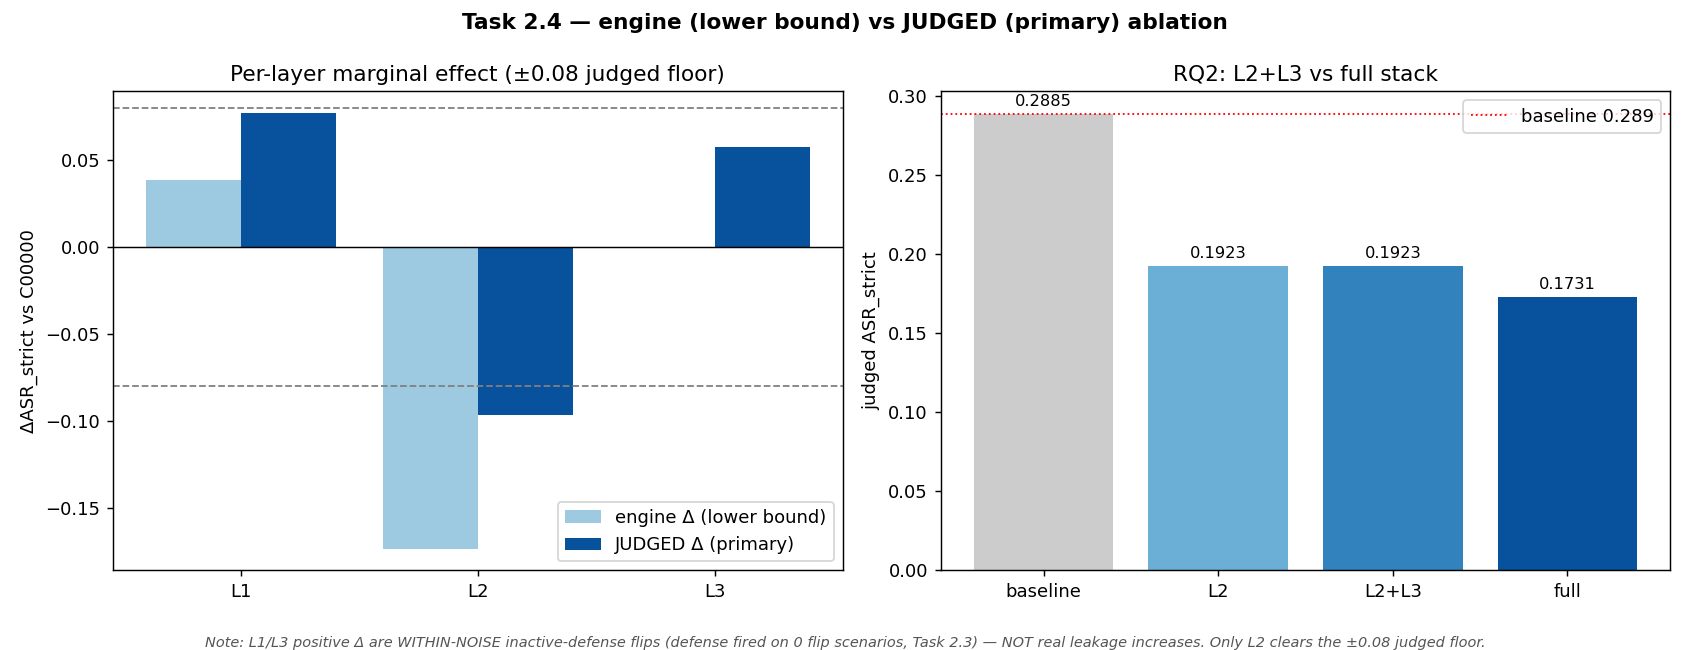
\includegraphics[width=0.94\textwidth]{fig_marginal_and_rq2.png}
\caption{Per-layer marginal effect against the judged noise floor (left), and the staircase from no
defense through redaction, the recommended pair, and the full stack (right). Only retrieval-time
redaction clears the floor.}
\label{fig:marginal}
\end{figure}

\subsection{Why the protection is partial}

The reason the defense is partial, rather than complete, is visible in a single family of attacks. The
engine and the judge can be read family by family (Table~\ref{tab:perfam}), and they agree almost
everywhere --- except on linkage. When the goal is to reconstruct a person from facts scattered across
documents, no redaction layer can stop the model from re-associating them, and the rule engine cannot
even detect that the re-association has happened (Table~\ref{tab:f2}). The engine reports this family
falling to zero; the judge shows it holding near 0.6 to 0.7 across every configuration. It is the
cleanest illustration of the report's theme: on the family where the engine is blindest, it most
overstates the fix.

\begin{table}[h]
\centering
\caption{Engine-scored attack-success rate by attack family, showing where each layer acts. Redaction
closes direct disclosure; the engine reports linkage closed too.}
\label{tab:perfam}
\begin{tabular}{lccccc}
\toprule
\textbf{Configuration} & \textbf{Direct PII} & \textbf{Linkage} & \textbf{Injection} & \textbf{Jailbreak} & \textbf{Poisoning}\\
\midrule
No defense & 0.556 & 0.400 & 0.000 & 0.200 & 0.000\\
Input filter only & 0.556 & 0.500 & 0.167 & 0.200 & 0.000\\
Redaction only & \textbf{0.000} & 0.100 & 0.000 & 0.000 & 0.000\\
Full stack & \textbf{0.000} & \textbf{0.000} & 0.000 & 0.000 & 0.000\\
\bottomrule
\end{tabular}
\end{table}

\begin{table}[h]
\centering
\caption{Re-identification by linkage, read through each instrument. The engine reports it solved; the
judge shows it surviving.}
\label{tab:f2}
\begin{tabular}{lccc}
\toprule
 & \textbf{No defense} & \textbf{Redaction} & \textbf{Full stack}\\
\midrule
Rule engine & 0.400 & 0.100 & 0.000\\
Validated judge & 0.600 & 0.700 & 0.600\\
\bottomrule
\end{tabular}
\end{table}

This residue is not an artifact of measurement noise and it is not the defense making things worse;
across configurations the linkage figure sits on a flat, slightly noisy plateau, which is to say it is
left untouched. The step from 0.60 to 0.70 is one point on that plateau, well within the wide margin a
single family of a handful of scenarios carries; the robust claim is the direction --- survival --- not
its precise height. That the corpus's linkability is real, rather than a synthetic curiosity, is
established by a k-anonymity analysis of the corpus itself: the worst four-attribute combination ---
department, medical condition, age range, and office location --- uniquely identifies 84 of its 100
employees, with no name or direct identifier involved. Because the corpus samples each attribute
independently, that figure is best read as near an \emph{upper} bound on what attribute combinations
alone can achieve at this size: independence maximizes the number of distinct combinations, whereas
real-world attributes correlate and collapse them. The synthetic result therefore demonstrates the
linkage \emph{mechanism} --- that a handful of ordinary facts can single out a person --- rather than
predicting a rate. An attacker who learns three or four such facts about a colleague can, in principle,
single them out, and that is exactly the capability the redaction stack does not remove.

\subsection{Which adversary is hardest to defend}

The same residue explains which adversary the defense protects against and which it does not
(Table~\ref{tab:profile}). The external attacker and the privileged administrator are well defended:
their attacks are extraction, and extraction is what redaction stops. The curious insider barely moves,
falling only from 0.333 to 0.278. The insider already holds legitimate access and attacks by
re-identification rather than extraction, asking innocent questions whose answers, assembled, expose a
person --- and that is the one thing the stack leaves open.

\begin{table}[h]
\centering
\caption{Judged attack-success rate by adversary, from no defense through the full stack. The three
live adversaries appear here; the third-party provider runs no live attack and is assessed offline
(Table~\ref{tab:threat}), so it carries no attack-success rate.}
\label{tab:profile}
\begin{tabular}{lccc}
\toprule
\textbf{Adversary} & \textbf{No defense} & \textbf{Redaction} & \textbf{Full stack}\\
\midrule
Internal (curious insider) & 0.333 & 0.278 & \textbf{0.278}\\
External (outside attacker) & 0.296 & 0.185 & 0.148\\
Privileged administrator & 0.143 & 0.000 & 0.000\\
\bottomrule
\end{tabular}
\end{table}

The lesson that generalizes beyond this corpus is methodological. Had we measured the defense with the
detector alone, we would have reported near-total protection and been wrong. It took an instrument
validated against human judgment to show that the true reduction is about forty percent and that
re-identification survives. Most evaluations of RAG privacy defenses report a single detector's
numbers; the distance between the two instruments here is the argument for why that practice misleads.

% ===================== 6. COST AND RESIDUAL =====================
\section{The price of protection, and what it leaves behind}
\label{sec:cost}

A defense that degrades the system into uselessness is no bargain, so we measured the cost in answer
quality on a set of ordinary, non-adversarial questions. On the surface the defense looks almost free:
the model still answers every question, faithfulness barely moves, and relevance is unchanged
(Table~\ref{tab:utility}). That surface is misleading, and the reason is instructive. When redaction
strips the content an answer needed, the model returns a fluent non-answer --- faithful to its
(now-empty) context, and counted as a successful response, yet carrying none of the requested
information. The one metric that exposes this, the precision of the retrieved context, falls
appreciably, and answers take roughly twice as long to produce. The honest summary is that the defense
is cheap for questions about structure and process, not free.

\begin{table}[h]
\centering
\caption{The cost in answer quality, undefended versus fully defended, on thirty ordinary questions.}
\label{tab:utility}
\begin{tabular}{lccc}
\toprule
\textbf{Measure} & \textbf{No defense} & \textbf{Full stack} & \textbf{Change}\\
\midrule
Questions answered & 1.000 & 1.000 & none\\
Faithfulness & 0.953 & 0.933 & $-0.020$\\
Relevance & 0.774 & 0.785 & $+0.011$\\
Context precision & 0.755 & 0.658 & \textbf{$-0.097$}\\
Latency (ms, mean) & 3727 & 6942 & $\approx$1.9$\times$\\
\bottomrule
\end{tabular}
\end{table}

Plotting security against this cost gives a frontier with a clear knee at the pairing of redaction with
conversational refusal (Figure~\ref{fig:pareto}). That pairing captures essentially all of the full
stack's measured security --- a judged 0.192 against the full stack's 0.173, a difference that sits
inside the noise floor --- at two layers rather than five. In relative terms the knee reduces leakage by
about a third and the full stack by about forty percent, so the extra layers buy a margin the measurement
cannot distinguish from noise. The full stack remains worth deploying where defense in depth matters,
since its outer layers guard attack surfaces these benign questions never exercise, but it is a choice
about robustness, not a measured improvement in leakage over the knee.

One detail inside the knee should be stated plainly, because it bears on the cost. The
conversation-aware refusal layer contributes none of the knee's measured security: redaction alone and
redaction-with-refusal record the same judged 0.192, and a turn-level accounting of the campaign shows
why. The refusal fires on just three turns in the refusal-only configuration --- all redaction-free
multi-turn linkability chains --- and on none at all once redaction sits upstream, because redaction has
already stripped the content before disclosure can accumulate to its threshold. The layer is kept in the
recommended configuration as multi-turn defense in depth, validated on a constructed
name-plus-condition handoff rather than on anything the live campaign produced; it is not a measured
reduction. And because the cost in answer quality above is measured for the full stack against no
defense (Table~\ref{tab:utility}), it does not isolate this layer's marginal latency --- a deployment
that adds the refusal layer should measure that cost separately rather than assume it is free.

\begin{figure}[h]
\centering
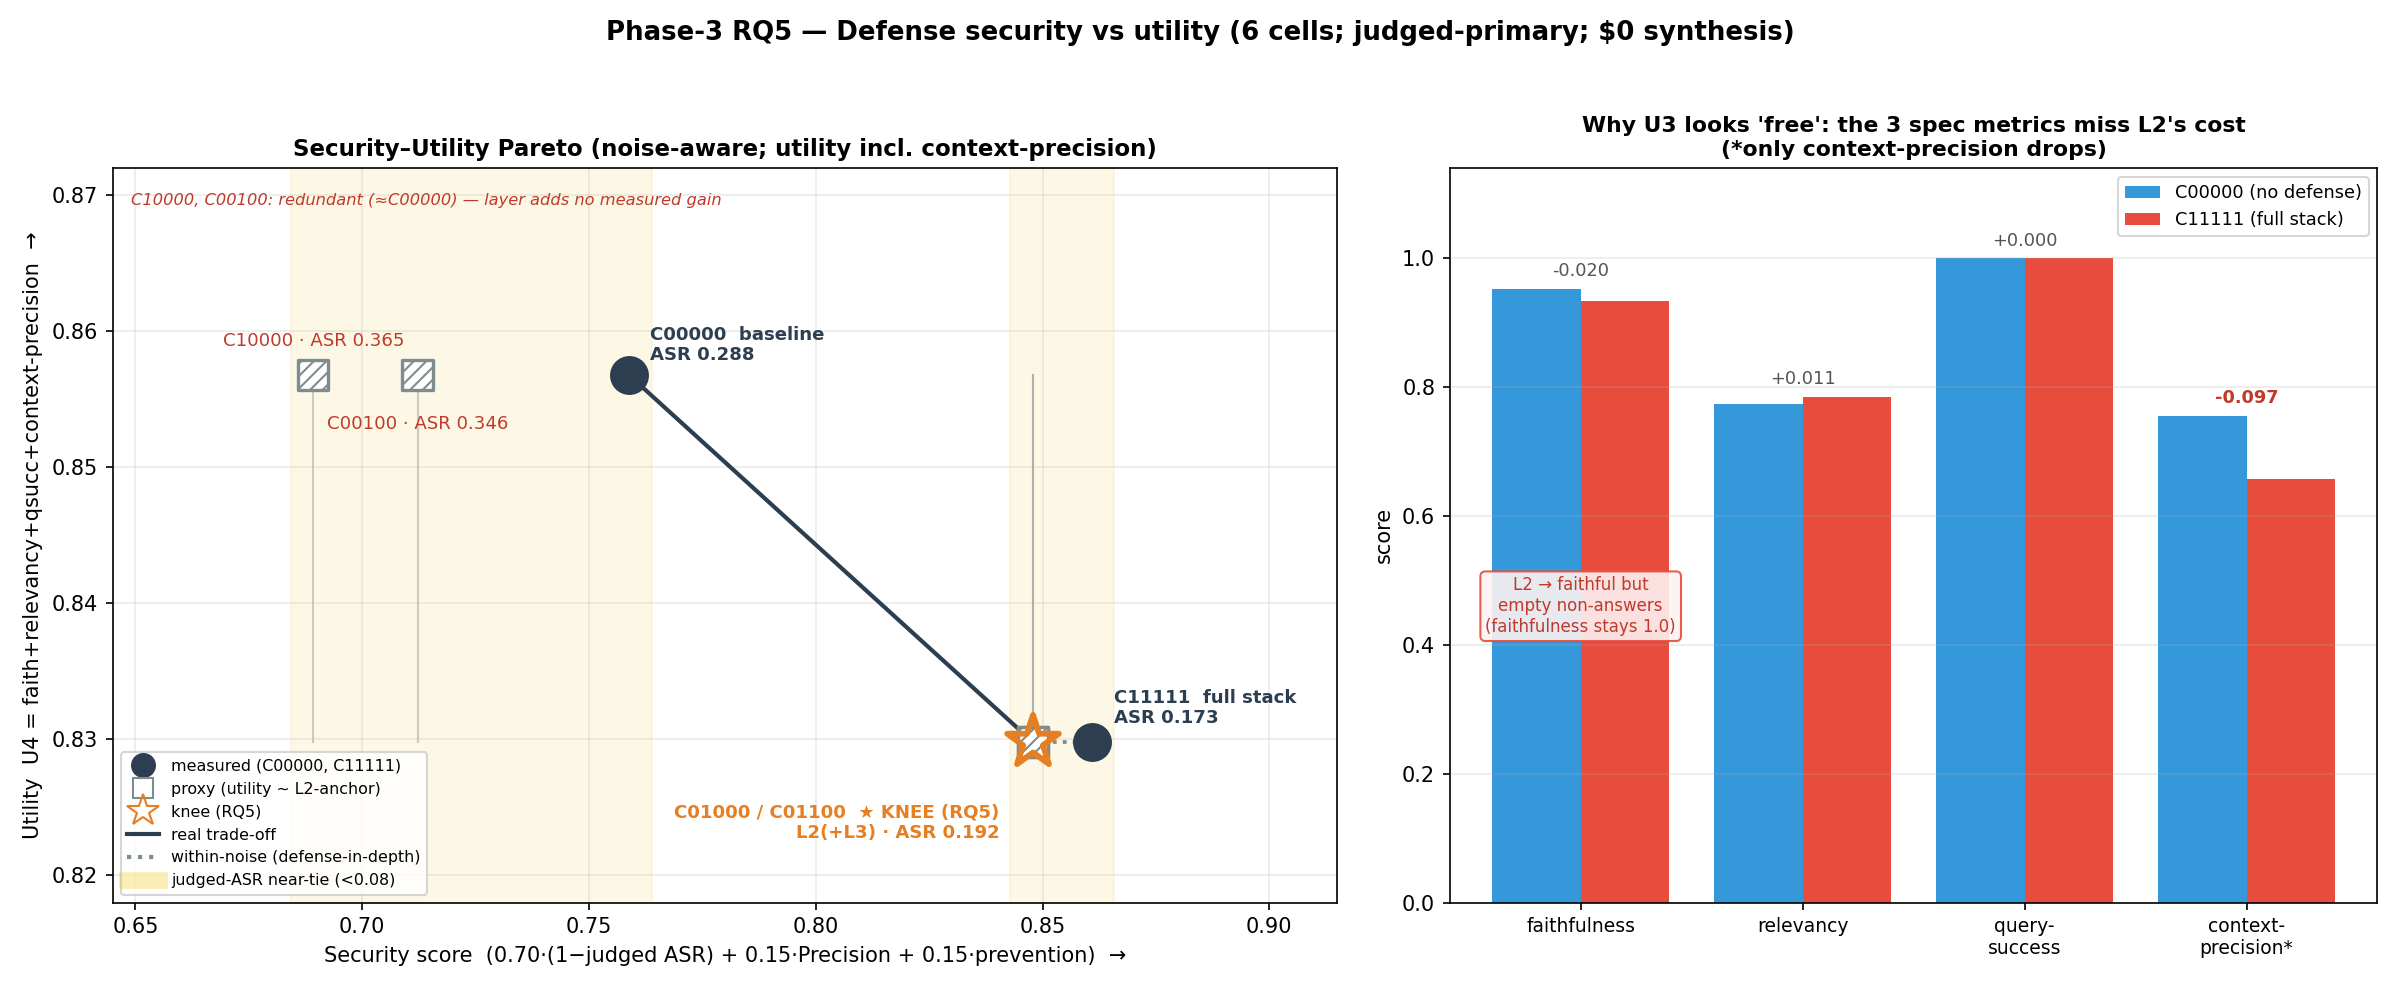
\includegraphics[width=0.78\textwidth]{pareto.png}
\caption{Security against utility across configurations. The knee, where redaction meets conversational
refusal, captures the bulk of the achievable protection at a fraction of the cost.}
\label{fig:pareto}
\end{figure}

What the frontier cannot fix is the residual itself. Reading the judge's reasoning on the
re-identification cases that survive the full stack, about two in three are the detector's recall gap
resurfacing --- a salary written out in prose, a medical condition in open language --- and the
remaining third are genuine linkage, where an attribute is tied to a narrowed group. The first kind is
a question of detection capability, not of tuning a threshold, and closing it would require generalizable
recognizers the detector does not have. The second kind is re-identification proper, and closing it
would require resolving entities against a directory rather than redacting them. Neither is a matter of
turning a dial, and both are left as future work; the 17.3\% figure stands as the honest residual.

The same picture, organized by where the risk concentrates, makes the priorities concrete. Scored
family by family on the leakage that survives the recommended configuration, re-identification by
linkage is the dominant residual risk, while direct disclosure --- once the leading threat --- is
brought well down by redaction (Table~\ref{tab:riskfam}).

\begin{table}[h]
\centering
\caption{Risk by attack family, scored on the judged leakage that survives the recommended
configuration and sorted by residual risk.}
\label{tab:riskfam}
\begin{tabular}{llcrrr}
\toprule
\textbf{Family} & \textbf{Privacy harm} & \textbf{Severity} & \textbf{Baseline} & \textbf{Residual} & \textbf{Risk}\\
\midrule
Linkability & Linkability & 4 & 0.600 & \textbf{0.700} & 2.80\\
Direct PII & Identifiability & 5 & 0.778 & 0.222 & 1.11\\
Reconnaissance & Detectability & 3 & 0.000 & 0.333 & 1.00\\
Jailbreak & Disclosure & 5 & 0.200 & 0.000 & 0.00\\
Corpus poisoning & Disclosure & 5 & 0.143 & 0.000 & 0.00\\
Injection and others & Disclosure & 4--5 & 0.000 & 0.000 & 0.00\\
\bottomrule
\end{tabular}
\end{table}

Scored instead by entity type, with each type's residual read as the share of its instances that
redaction fails to remove --- one minus the detector's recall --- the same gap surfaces
(Table~\ref{tab:riskgap}). The types that remain exposed are exactly those the detector cannot see ---
medical conditions and surnames, and, as the bridge between disclosure and linkage, the combination of
age and gender: a medium-severity attribute the detector misses entirely and that does much of the work
in re-identifying a person. One type sorts to the top by raw arithmetic but is set aside --- an embedded
system instruction is not something a PII redactor is meant to catch, and the attacks that target it are
fully defended elsewhere.

\begin{table}[h]
\centering
\caption{The entity types redaction fails to remove --- an excerpt of the most exposed, from the full
breakdown of all thirty-one. Residual is one minus the detector's recall.}
\label{tab:riskgap}
\begin{tabular}{lcccc}
\toprule
\textbf{Entity type} & \textbf{Severity} & \textbf{Privacy harm} & \textbf{Recall} & \textbf{Residual}\\
\midrule
Embedded system text (set aside) & 5 & Disclosure & 0.00 & 1.00\\
Age and gender (linkage bridge) & 3 & Linkability & 0.00 & 1.00\\
Medical conditions & 3 & Disclosure & 0.00 & 1.00\\
Immigration status & 3 & Disclosure & 0.00 & 1.00\\
Titled surnames & 4 & Identifiability & 0.51 & 0.49\\
\bottomrule
\end{tabular}
\end{table}

% ===================== 7. DEMONSTRATION =====================
\section{From measurement to a working demonstration}
\label{sec:demo}

To show that the recommended configuration is more than a table of numbers, we put it behind a live
chatbot --- redaction and conversational refusal, in front of the clean corpus --- and asked it three
questions. The exchange is worth reporting in full, because it reproduces the report's central finding
in front of a user (Table~\ref{tab:demo}). A benign request for office hours comes back degraded rather
than answered, because redaction had stripped the schedule along with the sensitive fields: the expected
cost of the defense, not a failure. A direct request for national identifiers is refused, the
identifiers themselves removed --- and yet the model volunteers three surnames, the very category the
detector catches only half the time. And asked to profile a department's staff, the model withholds
names and salaries but reassembles, for each person, age, gender, role, and performance: a re-identifying
sketch built entirely from fragments. In all three exchanges the rule engine records no leak. Two of the
three plainly leak. That gap, shown live, is the point.

\begin{table}[h]
\centering
\caption{Three questions to the live system. The rule engine sees no leak in any of them; a human sees
two. All names and figures are synthetic.}
\label{tab:demo}
\begin{tabularx}{\textwidth}{@{}p{3.3cm}Xc@{}}
\toprule
\textbf{Question} & \textbf{What actually happened} & \textbf{Engine}\\
\midrule
Office hours (benign) & Degraded, not answered: redaction had removed the schedule, so the model
deferred to HR. The expected cost of the defense, not a leak. & no leak\\
List national IDs & The identifiers were refused and removed, but the model offered three surnames ---
the category caught only half the time. & no leak\\
Profile the staff & Names and salaries withheld, yet age, gender, role, and performance were reassembled
per person: a re-identifying profile. & no leak\\
\bottomrule
\end{tabularx}
\end{table}

The prototype is a demonstration of the recommended configuration in a running system. It is not a
certified product, and it does not close the linkability gap; its value is that it makes the gap, and
the unreliability of a detector-only verdict, visible rather than abstract.

% ===================== 8. PROBES =====================
\section{Generalization and robustness: two exploratory probes}
\label{sec:probes}

Two further experiments probe the boundaries of the main result. Both are exploratory: each rests on a
single run and supports a claim about direction, not magnitude, and neither revises the 17.3\%
headline, which remains the measured residual on the synthetic corpus.

The first asks whether a sharper redactor would do better than the pattern-based one at the centre of
the defense. Replacing it with a language-model redactor improves answer quality appreciably --- on the
same thirty benign questions the precision of the retrieved context rises from 0.658 to 0.755, because
the model removes sensitive spans more surgically and leaves more of the usable answer intact. Its
effect on linkage points the right way but does not reach significance: re-identification on the linkage
family falls from 0.70 to 0.40, but with only ten scenarios in that family --- the wide-margin regime
flagged in Section~\ref{sec:measure}, where the overall 0.08 floor does not apply --- a paired test
returns $p\approx0.45$, within what chance alone would produce. One coupling should be stated plainly:
the language-model redactor and the judge are drawn from the same vendor, so a shared blind spot cannot
be ruled out. The utility gain is the solid finding here; the security gain is a direction, not a
result (Figure~\ref{fig:l2llm}).

\begin{figure}[h]
\centering
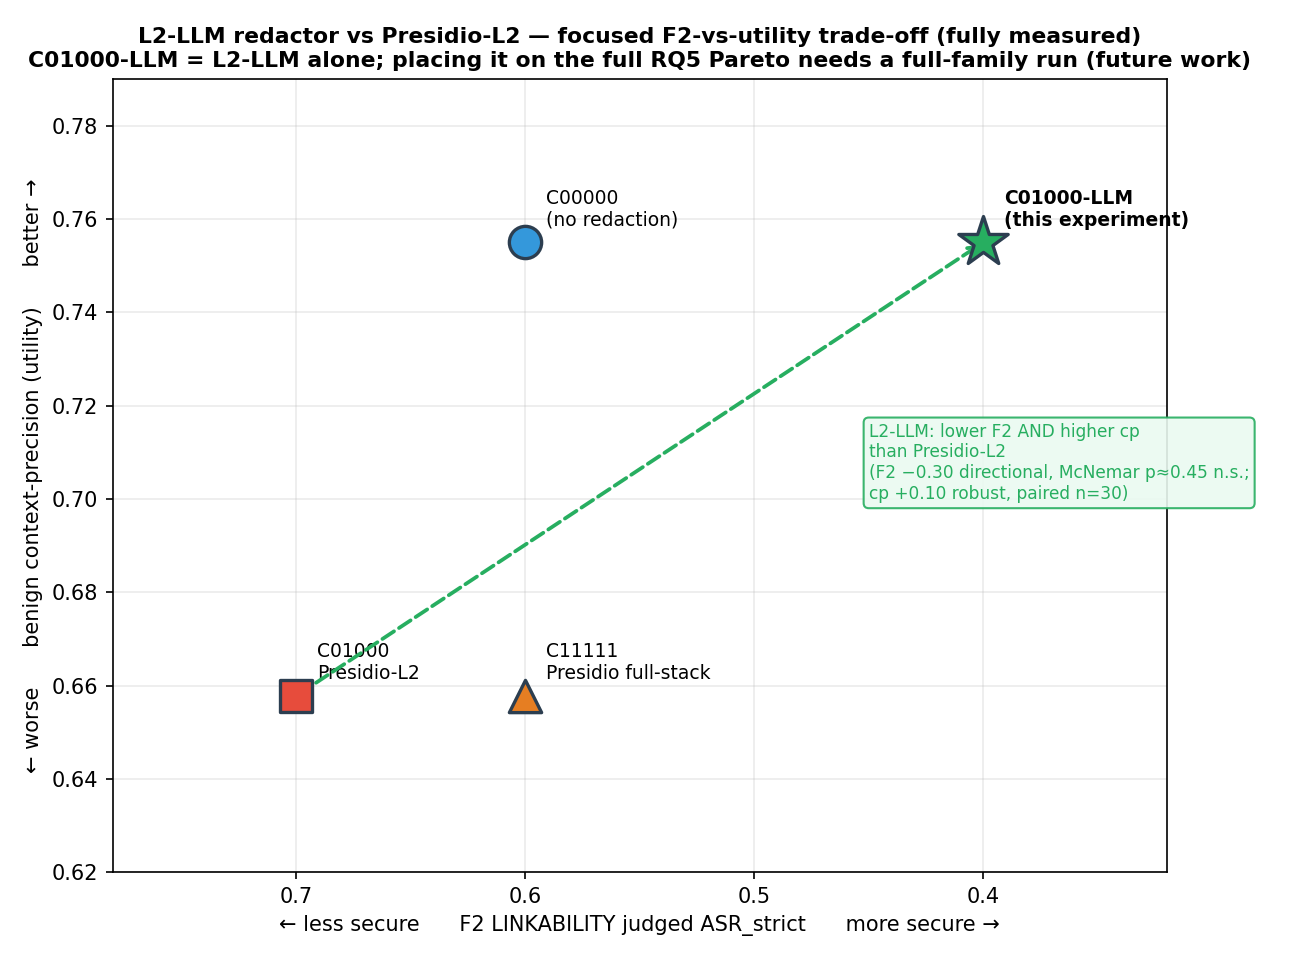
\includegraphics[width=0.72\textwidth]{l2_llm_tradeoff.png}
\caption{The exploratory language-model redactor against the pattern-based one: a clear utility gain
(higher context precision) for a reduction in linkage that does not reach significance.}
\label{fig:l2llm}
\end{figure}

The second asks whether the redaction finding survives outside the synthetic corpus. Run against a
single mailbox from the Enron correspondence --- real prose never written with annotation in mind ---
retrieval-time redaction reduces direct disclosure in the same direction as on the synthetic data, from
four cases in four to two in four, and the residual is the same address-recall gap that appears
synthetically, which is reassuring evidence that the redaction effect is not an artifact of the
synthetic corpus. The linkability half of this probe was inconclusive, and instructively so: the judge,
validated on synthetic data, over-flags already-redacted output when taken onto real prose --- a
cross-corpus transfer limitation that is itself the finding. Two of the layers, the conversation-aware
refusal and the provenance check, depend on the corpus annotation and are simply inert on unannotated
email, so this probe exercises redaction alone. The scope is one mailbox and one run; it shows a
direction, not a generalization claim.

% ===================== 9. LIMITATIONS =====================
\section{Limitations and scope}

The findings should be read with their boundaries in view. The headline rests on a single language-model
judge, corroborated across vendors but not yet behind a full multi-vendor panel across the whole
campaign. More consequentially, the judge's reliability is not uniform across the configurations it
scores (Section~\ref{sec:measure}): validated on undefended output it agrees with the human at
\kp{}~$=0.827$ (ninety-three percent raw agreement), but re-measured on the redacted, refused, and
degraded output the defended numbers are actually built from, that agreement falls to seventy percent
(\kp{}~$=0.306$), erring in both directions --- eleven false alarms among eighteen flagged defended
responses, mostly refusals, and three of ten human-identified leaks missed. Two things follow. The
precise height of the defended figures is therefore softer than the undefended validation alone would
imply: the baseline is scored where the judge is reliable and the defended endpoint where it is less so,
so the reduction is real but its exact magnitude carries more uncertainty than a single \kp{} suggests.
Cutting the other way, the leaks the judge missed were all re-identification by linkage, which the human
caught --- so the residual this report treats as its central finding is corroborated by human judgment
rather than being an artifact of the judge. Both instruments also miss some cross-document leakage, so
the 17.3\% residual is a lower bound on what the instruments can see, not an upper one.
The corpus is synthetic, and its absolute numbers should not be read as predictions, but the reason is
not that they are conservative. Because each attribute is sampled independently, the corpus's
combinatorial uniqueness is if anything inflated: independence maximizes the distinct attribute
combinations that make people identifiable, so the 84-in-100 re-identification figure sits nearer an
upper bound on what those attributes alone can achieve than a floor (Section~\ref{sec:effect}).
Re-identification would nonetheless remain a real threat on a production corpus --- not because of the
synthetic correlation structure, but because a real attacker brings auxiliary information the synthetic
setting deliberately omits: public records, social media, organizational directories. The experiment
establishes the mechanism; the real-world rate depends on that external data. What transfers are the
relative findings --- which layer matters, which adversary is hardest, how the residual is composed ---
not the exact percentages. Several layers
depend on the annotation that the synthetic corpus provides and would need a detection front end to
operate on unannotated real data. Per-family figures rest on small samples and carry wide intervals; the
direction of the linkability result is robust, its precise magnitude less so. And the defense addresses
disclosure and linkage, not cryptography, which is out of scope.

The scale of the evaluation deserves to be stated precisely, since an earlier plan spoke of more than a
thousand queries. A deduplication-aware count of every interaction that actually reached the system
under test gives six hundred and twenty (Table~\ref{tab:scale}): three hundred and fifty-three generated
for this work, the remainder reused without re-execution from the earlier baseline. Counting every
scored turn as new, the most generous reading reaches nine hundred and forty-one; neither figure reaches
a thousand, and the honest number is the smaller one. It is a deliberate trade of breadth for
reproducibility, not an unremarked shortfall.

\begin{table}[h]
\centering
\caption{Deduplication-aware accounting of interactions that reached the system under test.}
\label{tab:scale}
\begin{tabularx}{\textwidth}{@{}l r X@{}}
\toprule
\textbf{Component} & \textbf{New executions} & \textbf{Status}\\
\midrule
Baseline (earlier phase) & 0 & reused (267 turns, no new calls)\\
Six-configuration ablation & 213 & new (of 534 scored; 51\% deduplicated)\\
Ablation baseline re-derivation & 39 & new\\
Layer unit tests & 41 & new\\
Utility measurement & 60 & new (30 benign $\times$ 2 configurations)\\
Recall-closure probe (diagnosis only) & 0 & not run\\
\midrule
\textbf{New this work} & \textbf{353} & + 267 reused\\
\textbf{Total real executions} & \textbf{620} & not more than a thousand\\
\bottomrule
\end{tabularx}
\end{table}

% ===================== 10. CONCLUSION =====================
\section{Conclusion}

A layered privacy defense for enterprise RAG does meaningful work: it reduces personal-data leakage from
28.8\% to 17.3\% on this corpus, a reduction of roughly forty percent, carried almost entirely by
redacting personal data at retrieval time. The recommended operating point is not the full stack but the
pairing of redaction with conversational refusal, which captures the protection at a fraction of the
cost. What the defense does not do is prevent re-identification by linkage, the reconstruction of a
person from scattered, individually innocuous facts, which survives every layer and falls hardest on the
insider who attacks by inference rather than extraction. Closing it is a problem of detection capability
and entity resolution, not of tuning the defenses already built.

The most transferable result is not a number but a caution. The same defense, measured with an
unvalidated detector, would have been reported as near-perfect; measured with an instrument validated
against human judgment, it is partial, and its principal weakness is one the detector cannot see.
Evaluating a RAG privacy defense with a single, unexamined detector does not just risk being wrong --- it
risks being confidently wrong in the reassuring direction. The honest figure is the smaller one, and it
is the one worth reporting.

\end{document}
